
\documentclass[runningheads]{llncs}
\usepackage{graphicx}
\usepackage[utf8]{inputenc}
\usepackage{fancyhdr}

\usepackage{tabularx}
\usepackage{booktabs}
 
\pagestyle{fancy}
\fancyhf{}
\fancyhf{}
\rhead{ULEAM}
\lhead{Universidad Laica "Eloy Alfaro" de Manabí}
\rfoot{\thepage}

% If you use the hyperref package, please uncomment the following line
% to display URLs in blue roman font according to Springer's eBook style:
% \renewcommand\UrlFont{\color{blue}\rmfamily}

\begin{document}
%
\title{Impacto de la inteligencia artificial en las redes sociales digitales}

%\titlerunning{Abbreviated paper title}
% If the paper title is too long for the running head, you can set
% an abbreviated paper title here
%
\author{Estudiante: Daza Santos Silvana Yanira}
%
\authorrunning{Universidad Laica "Eloy Alfaro" de Manabí}
% First names are abbreviated in the running head.
% If there are more than two authors, 'et al.' is used.
%
\institute{Universidad Laica "Eloy Alfaro" de Manabí\\
\email{e1317972253@live.uleam.edu.ec}}
%
\maketitle 
%%%%%%%%%%%%%%%%%%%%%%%%%%%%%%%%%%%%%%%%%%%%%%%%%%%%%%%%%%%%%%%%%
%%                            ABSTRACT                         %%
%%%%%%%%%%%%%%%%%%%%%%%%%%%%%%%%%%%%%%%%%%%%%%%%%%%%%%%%%%%%%%%%%
\begin{abstract}
La inteligencia artificial (IA) en las redes sociales digitales presenta tanto ventajas como desventajas, un desafío importante es la toma de decisiones automatizadas, que implica cuestiones éticas relacionadas con la privacidad de datos y la responsabilidad. Por esto, es crucial que la comunicación digital en estos entornos beneficie a la sociedad y que las máquinas se limiten a ser herramientas que conecten el mundo digital con las personas. A futuro, se busca desarrollar una inteligencia que iguale a la humana, enfocándose siempre en su uso responsable y beneficioso.
\keywords{Inteligencia artificial; redes sociales digitales; algoritmos, comunicación 
digital }
\end{abstract}
%
%%%%%%%%%%%%%%%%%%%%%%%%%%%%%%%%%%%%%%%%%%%%%%%%%%%%%%%%%%%%%%%%%
%%                        INTRODUCCIÓN                         %%
%%%%%%%%%%%%%%%%%%%%%%%%%%%%%%%%%%%%%%%%%%%%%%%%%%%%%%%%%%%%%%%%%
\section{Introducción}
Actualmente, las personas se conectan e interactúan a través de redes sociales digitales (RSD), donde la Inteligencia Artificial (IA) ha revolucionado la comunicación digital. Las RSD han evolucionado de simples plataformas de interacción a convertirse en motores de recomendación, espacios de expresión y fuentes de información para millones de usuarios en todo el mundo. La IA juega un papel fundamental en esta transformación, mejorando la eficiencia, personalización y seguridad de estas redes.
La interacción entre IA y RSD se evidencia en diversos aspectos; por ejemplo, los algoritmos de IA optimizan la presentación de contenidos, mostrando a los usuarios publicaciones, videos y anuncios que se ajustan a sus gustos y comportamientos en línea, fomentando así una mayor participación y alcance efectivo de las audiencias. Sin embargo, este avance también plantea preocupaciones sobre privacidad, ética y la posible polarización de opiniones. 
El uso de algoritmos de IA puede crear filtros que limitan la información que los usuarios ven, reforzando sus creencias existentes. Además, la recopilación de datos personales para personalizar el contenido genera inquietudes sobre privacidad y seguridad en línea. En todas las áreas del mundo globalizado, la IA ha impactado significativamente, especialmente en las RSD, cambiando cómo se comunica e interactúa en el entorno digital.
La IA influye en la forma de procesar la información en distintos campos, como el procesamiento del lenguaje, donde permite a las máquinas comprender e interpretar el lenguaje humano. También facilita el análisis de datos en RSD para entender los sentimientos de los usuarios y generar contenido de manera eficiente. En general, la IA está redefiniendo la comunicación en personas e instituciones, ofreciendo personalización, automatización y sistematización, pero también presenta desafíos éticos y de seguridad en la evolución de la tecnología.

%%%%%%%%%%%%%%%%%%%%%%%%%%%%%%%%%%%%%%%%%%%%%%%%%%%%%%%%%%%%%%%%%
%%                      ESTADO DEL ARTE                        %%
%%%%%%%%%%%%%%%%%%%%%%%%%%%%%%%%%%%%%%%%%%%%%%%%%%%%%%%%%%%%%%%%%
\section{Planteamiento}
La evolución de la inteligencia artificial (IA) ha sido gradual, comenzando en 1956 con el Dartmouth Workshop, donde se establecieron las bases para su estudio. A lo largo del tiempo, la IA ha enfrentado desafíos y avances, desde los primeros sistemas de programación como Lisp hasta el desarrollo de sistemas expertos y redes neuronales. Durante las décadas de 1970 y 1980, la falta de avances condujo al "invierno de la IA", pero luego experimentó un resurgimiento con el aprendizaje automático y el procesamiento del lenguaje natural. En la actualidad, la IA ha crecido significativamente gracias a la disponibilidad de grandes cantidades de datos y algoritmos avanzados, impactando diversos campos como la computación, la robótica y las redes sociales digitales (RSD).
En las RSD, la IA se utiliza para personalizar contenido, mejorar la interacción con usuarios a través de chatbots y combatir problemas como la desinformación y el discurso de odio. Plataformas como Facebook, TikTok e Instagram emplean algoritmos que analizan el comportamiento de los usuarios para ofrecer contenido relevante. Aunque la IA ha transformado la comunicación digital, también plantea desafíos éticos y de privacidad, especialmente en el manejo de datos personales.
A pesar de estos desafíos, la IA no debe verse como competencia de la inteligencia humana, sino como una herramienta complementaria que puede combinarse con la creatividad y empatía humana. La relación entre la IA y las RSD sigue evolucionando, y es fundamental que su desarrollo se enfoque en el bienestar social, asegurando una gestión responsable y ética de la tecnología en las plataformas digitales.

%%%%%%%%%%%%%%%%%%%%%%%%%%%%%%%%%%%%%%%%%%%%%%%%%%%%%%%%%%%%%%%%%
%%                        MARCO TEÓRICO                        %%
%%%%%%%%%%%%%%%%%%%%%%%%%%%%%%%%%%%%%%%%%%%%%%%%%%%%%%%%%%%%%%%%%
\section{Metodología}
En el ámbito de la inteligencia artificial (IA) y las redes sociales digitales, la netnografía se utiliza para estudiar el comportamiento, las interacciones y las dinámicas culturales en línea. Este método se ha aplicado para analizar las emociones y percepciones de los usuarios sobre temas publicados en las redes sociales, identificando tendencias y patrones de flujo de información en la cultura digital. 
La netnografía se convierte en una herramienta clave para entender y aprovechar las opiniones y comportamientos en el entorno digital. Esto permite a las organizaciones adaptarse mejor a las dinámicas de las redes sociales, tomar decisiones basadas en datos y desarrollar estrategias efectivas en un entorno digital que cambia constantemente.

Dentro de las RSD se presentan algoritmos con la IA determinados en la siguiente 
ilustración:

\begin{figure}[h!]
            \centering
            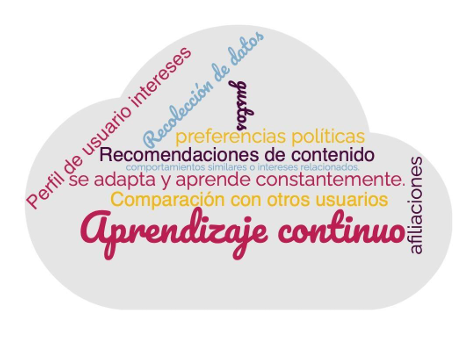
\includegraphics[width=0.5\linewidth]{ia.png}
            \caption{Resultados de algoritmos con IA en las RDS}
            \label{fig:enter-label}
\end{figure}
%%%%%%%%%%%%%%%%%%%%%%%%%%%%%%%%%%%%%%%%%%%%%%%%%%%%%%%%%%%%%%%%%
%%                  EXPLICACIÓN DEL CÓDIGO                     %%
%%%%%%%%%%%%%%%%%%%%%%%%%%%%%%%%%%%%%%%%%%%%%%%%%%%%%%%%%%%%%%%%%
\section{Discusión y conclusiones}
El análisis de la influencia de la Inteligencia Artificial (IA) en las redes sociales digitales revela un panorama complejo con múltiples facetas.


\begin{table}[h!]
\centering
\begin{tabularx}{\textwidth}{|X|X|X|}
\hline
\textbf{Ventajas} & \textbf{Desventajas} & \textbf{Efectos positivos y desafiantes de la IA en las RSD} \\
\hline
Personalización de contenido. & Burbujas de filtro y polarización: solo ver información que coinciden con las preferencias. & Avances en la atención médica, identificar Enfermedades. \\
\hline
Eficiencia en la moderación. & Falta de transparencia en las decisiones algorítmicas, no hay equidad ni imparcialidad. & Mejora en la toma de decisiones con las grandes cantidades de datos BIG DATA \\
\hline
Análisis de sentimiento. & Dependencia excesiva de la IA: Puede generar espacios en donde no ayude a la crítica y análisis. & Avances en la movilidad de forma segura y eficiente. \\
\hline
Detección de noticias falsas. & Privacidad y seguridad. Los algoritmos pueden ser generados con efectos negativos. & Personalización y Recomendación. \\
\hline
Traducción automática, comunicación digital en diferentes idiomas, alcance digital mundial. & Desempleo. & Automatización de tareas repetitivas. \\
\hline
\end{tabularx}
\caption{Impacto de la Inteligencia Artificial en las Redes Sociales Digitales}
\label{tab:impacto_ia}
\end{table}
La inteligencia artificial (IA) en las redes sociales digitales (RSD) permite personalizar la experiencia del usuario, fomentando su participación y compromiso. A pesar de sus beneficios, también genera preocupaciones sobre las "burbujas de filtro", donde los usuarios quedan expuestos a contenido repetitivo, afectando su interacción. Es crucial usar estas herramientas de manera ética y transparente. La IA aporta mejoras en la experiencia de usuario, eficiencia de las plataformas y beneficios tanto para usuarios como para empresas.
Sin embargo, la IA puede provocar la automatización de trabajos, desplazando a trabajadores en ciertas industrias, lo que plantea la necesidad de reentrenamiento laboral. También surgen preocupaciones sobre la privacidad y seguridad, ya que la recopilación de datos personales por parte de la IA puede poner en riesgo la información de los usuarios.
Además, los sesgos en los algoritmos de IA pueden llevar a discriminación en las decisiones automatizadas. La brecha digital se amplía, afectando a quienes no tienen acceso a estas tecnologías y exacerbando las desigualdades sociales y económicas. Los desafíos éticos relacionados con la IA en las RSD también incluyen efectos negativos en la salud mental, como la adicción y la ansiedad. Por último, la seguridad en línea es un riesgo, ya que los sistemas basados en IA pueden ser vulnerables a ciberataques, con consecuencias perjudiciales para la sociedad.
%%%%%%%%%%%%%%%%%%%%%%%%%%%%%%%%%%%%%%%%%%%%%%%%%%%%%%%%%%%%%%%%%
%%                       BIBLIOGRAFÍA                          %%
%%%%%%%%%%%%%%%%%%%%%%%%%%%%%%%%%%%%%%%%%%%%%%%%%%%%%%%%%%%%%%%%%
% \bibliographystyle{splncs04}
% \bibliography{mybibliography}

\begin{thebibliography}{8}
\bibitem{ref_article1}
Clarenc, C. A. (2011). Nociones de cibercultura y literatura. Lulu Com. 
Kahney, L. (2019). Tim Cook: The genius who took Apple to the next level. Penguin 
Business. 

\bibitem{ref_lncs1}
Li, F. F. (2023). The worlds I see: Curiosity, exploration, and discovery at the dawn of AI. Moment of Lift Books; Flatiron Books.

\bibitem{ref_book1}
Minsky, M. L. (2010). La máquina de las emociones: Sentido común, inteligencia artificial y el futuro de la mente humana (1a. ed). Debate

\bibitem{ref_proc1}
Turing, A.  M.  (2016).  ¿Puede pensar una máquina?  Createspace  Independent 
Publishing Platform. 

\bibitem{ref_url1}
Universidad     
Central.(2013). Manual     de     Estilo.     Manual     de     Estilo. 
https://www.ucentral.edu.co/editorial/recursos-para-escritura
\end{thebibliography}

\end{document}
